\subsection{\textcolor{red}{Database Handling}}

Based on our previous discussion of using the \m{Utility} class through its static methods, we can also update the \m{DatabaseHandler} to use static methods too, which are more efficient in Python. This involves just removing the references to \m{self}.


\subsection{\textcolor{red}{Optimisation}}

One of the things that we will be improving in the project is optimisation. We need to be able to run many frames per second and therefore, we need to be able to optimise the code. In order to do this, we will use the package \m{Cython}. In order to do this, we will compile all of the classes that we have written in order to make them more efficient to prevent excessive recompilation.
\vs

To do this, we can create a \m{setup.py} file, and convert all of our files in to \m{.pyx} files. The setup file is as follows for each \m{.pyx} file that we want to use.

\begin{mpy}
import cython
from setuptools import setup

from Cython.Build import cythonize

setup(ext_modules = cythonize("utils.pyx"))
\end{mpy}

Running this code, we get some new files, namely \m{utils.c} and \m{utils.cp310-win_amd64.pyd}. This still functions exactly like a normal Python class however, and we still retain all of the functiosn that we had in the original class.

\tbc

\subsection{\textcolor{red}{Game Loop HUD}}

The Heads-up Display, will just be showing the score for each team, and the total amount of time left in the game. This will be done by tracking the amount of time that has passed in seconds, and then writing it to the screen using the button class we created. The score will be created using two more buttons on either side.

\vs
However, before that can happen we need to find a way of computing the score. To do that we will simply use a for loop. However, since one already exists in our code, we can use that but add another line to it.

\vs
\begin{mpy}
            #Render players as needed
            for i, player in enumerate(self.players, 0):
                player.render(self.display, self.player1.position, self.SCREEN_DIMS, zoom)

                self.scores[player.team] += deltaDamageCredit[player] + 50 * deltaEliminationCredit[player] - 50*deltaDeathCredit[player]

\end{mpy}

This can be done by adding text renders to the \m{GameLoop} class. We will create a new function. 

\begin{mpy}
    def drawHUD(self):
        #Find remaining time
        currentTime = time.time()
        if currentTime - self.startTime >= self.maxTime:
            return False

        timeRemaining = int(300 - (currentTime - self.startTime))

        minutesRemaining = timeRemaining // 60
        secondsRemaining = timeRemaining % 60

        #Render time text
        time_text_surface, time_text_rect = text_font.render(str(minutesRemaining) + ":" + str(secondsRemaining), 
            fgcolor=(255, 255, 255), bgcolor=(0, 0, 0))

        #Set position on the screen
        time_text_rect.center = [self.SCREEN_DIMS[0]//2, 50]

        #Draw background rectangle
        pygame.draw.rect(self.display, (0,0,0), self.time_rect)

        self.display.blit(time_text_surface, time_text_rect)

        #Scores for each team
        #Team 1
        score1_text_surface, score1_text_rect = text_font.render(str(self.scores[0]), 
            fgcolor=(255, 255, 255), bgcolor=(0, 0, 255))

        score1_text_rect.center = self.score_1_rect.center
        pygame.draw.rect(self.display, (0, 0, 255), self.score_1_rect)
        self.display.blit(score1_text_surface, score1_text_rect)

        #Team 2
        score2_text_surface, score2_text_rect = text_font.render(str(self.scores[1]), 
            fgcolor=(255, 255, 255), bgcolor=(255, 0, 0))

        score2_text_rect.center = self.score_2_rect.center
        pygame.draw.rect(self.display, (255, 0, 0), self.score_2_rect)
        self.display.blit(score2_text_surface, score2_text_rect)

        return True

\end{mpy}

This code will produce the following output. As you can the score updates based on the things that are happening within the game.


\begin{figure}[H]
        \centering
        {
        \setlength{\fboxsep}{0pt}%
        \setlength{\fboxrule}{1pt}%
        \fbox{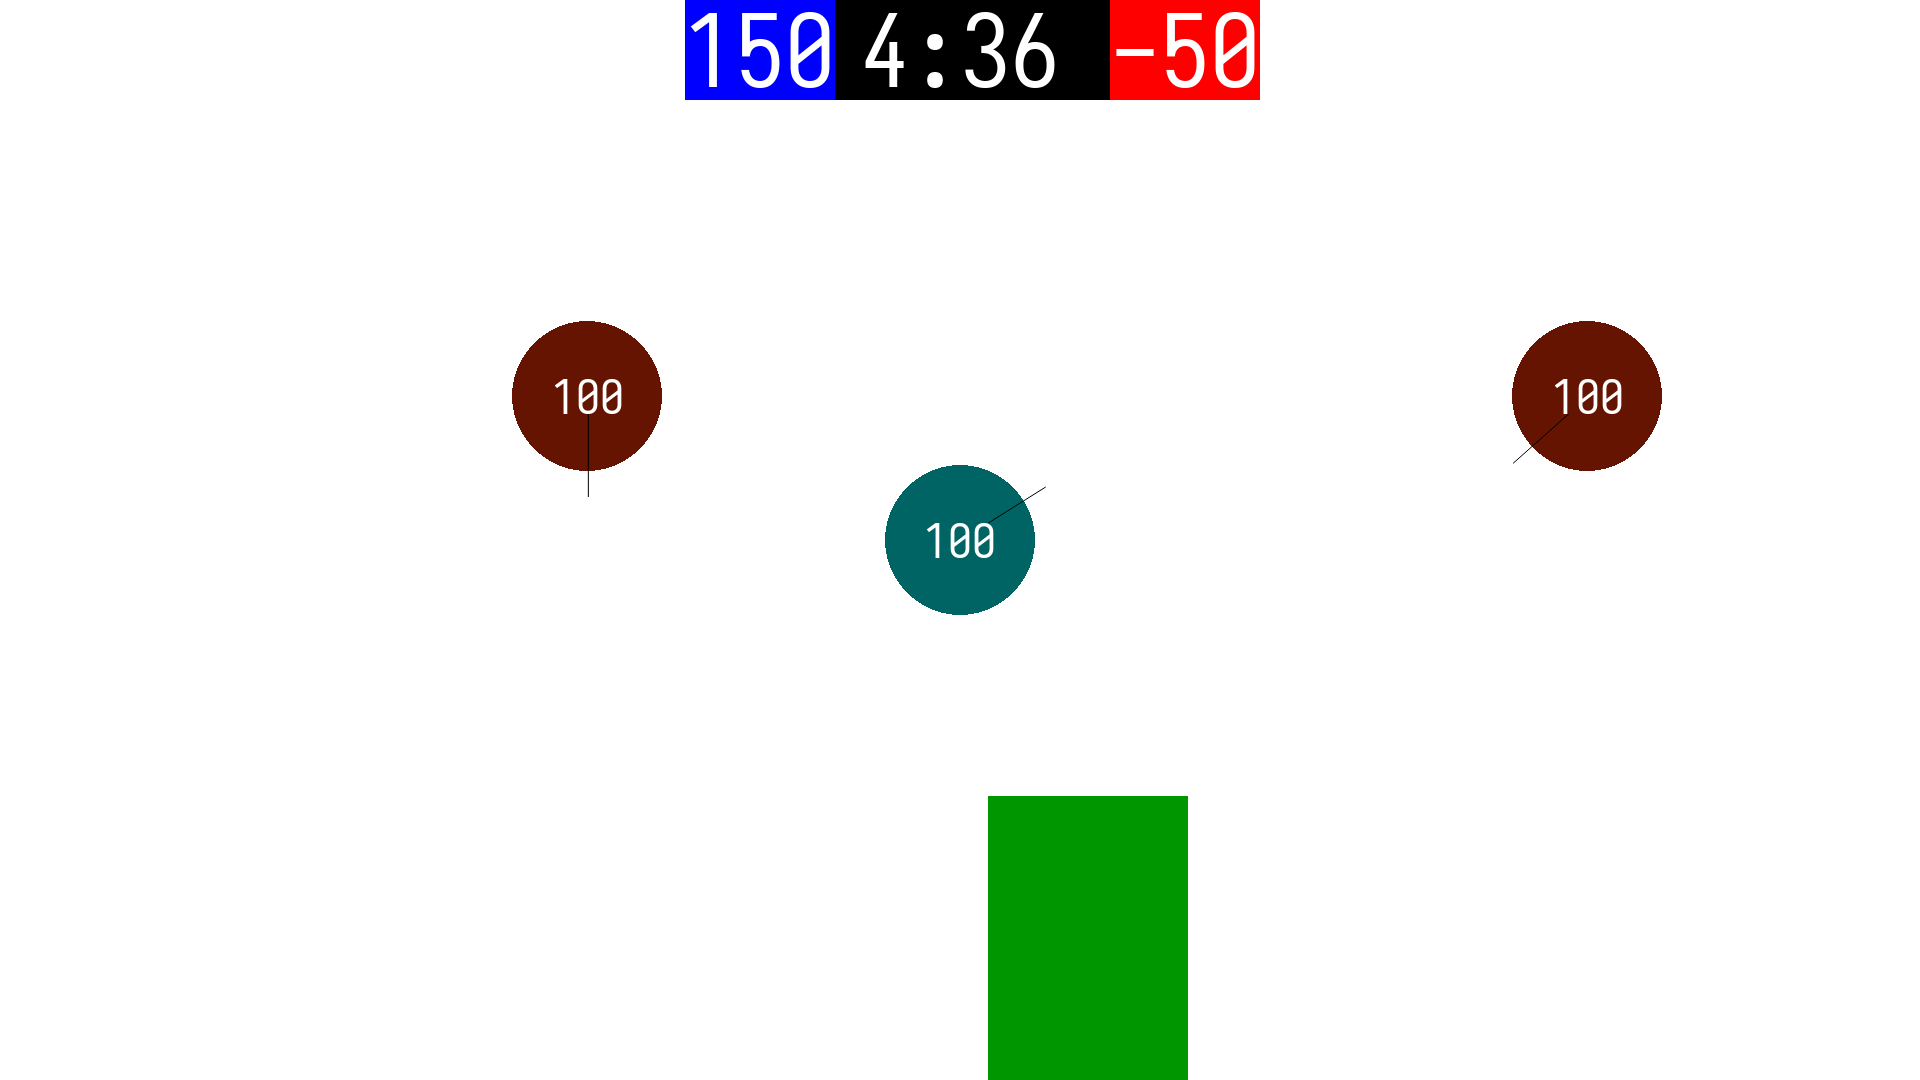
\includegraphics[width=\linewidth]{Development/Images/game_loop_2_1_hud.png}}
        }
        \caption{A screen capture of the map being zoomed out via the bound buttons}
        \label{fig:game_loop_2_1_hud}
\end{figure}

\vs
With this done, we can now return the total score for each team at the end of the game.


\subsection{\textcolor{red}{Environment}}

The first thing we need to do before starting doing any AI is to create the environment. This involves converting our game loop into something that can be run by a program which is then used to train the AI.

\vs
The first step in doing this is to remove all of the rendering functions. This is because we aren't rendering the game anymore and so we can just remove it. However, for the moment we will just create a copy of the game and comment out all of the rendering references in the main game loops. We only need the \m{GameLoop.run()} function primarily. 

\vs

Here I have imported all of the libaries that I need to run my training environment.

\begin{mpy}
from pettingzoo import ParallelEnv
from momentum_env.weapon import Weapon, Shotgun, AssaultRifle, SniperRifle
from momentum_env.player import Player
from momentum_env.block import Block
from momentum_env.utils import Utility as U
import numpy as np

import functools
from copy import copy

from gymnasium.spaces import Discrete, MultiBinary, Dict, Box, Tuple
from gymnasium.spaces.utils import flatten_space
from math import pi
\end{mpy}

Now, I need to create my environment's constructor. For this, I have just removed all of the calls to rendering and anything related to graphics. This has most of the same code as the constructor from the \m{GameLoop} class.

\begin{mpy}
class Momentum(ParallelEnv):
    metadata = {
        "name": "momentum_env",
    }

    def __init__(self, set_seed=42):
        self.REFRESH_RATE = 240
        self.dt = 1 / self.REFRESH_RATE

        # Team 1
        self.player1 = Player([1000, 3000], [0, -1], 0, Shotgun(self.REFRESH_RATE))
        self.player2 = Player([2000, 3000], [0, -1], 0, AssaultRifle(self.REFRESH_RATE)
        )
        self.player3 = Player([3000, 3000], [0, -1], 0, SniperRifle(self.REFRESH_RATE)
        )

        # Team 2
        self.player4 = Player([3000, 1000], [0, 1], 1, Shotgun(self.REFRESH_RATE))
        self.player5 = Player([2000, 1000], [0, 1], 1, AssaultRifle(self.REFRESH_RATE))
        self.player6 = Player([1000, 1000], [0, 1], 1, SniperRifle(self.REFRESH_RATE))

        # Contains all of the players in the game
        self.players = [self.player1, self.player2, self.player3, self.player4, self.player5, self.player6]

        #Blocks
        self.block1 = Block([1500, 2000], 200, 1200)
        self.block2 = Block([2500, 2000], 200, 1200)
        #self.block3 = Block([1000, 2000], 400, 400)
        #self.block4 = Block([2000, 2000], 400, 400)
        #self.block5 = Block([3000, 2000], 400, 400)

        #List of all blocks
        self.blocks = [self.block1, self.block2]#, self.block3, self.block4, self.block5]

        #Set countdowns
        self.countdowns = {p: 0 for p in self.players}
\end{mpy}

Furthermore, we want to be able to interchange between player instances and labels and so we will use dictionaries since they are perfect for this purpose. We will also create an array of all of the agents, so that the AI code can find the agents that we want to use.


\begin{mpy}
        #Access player object using string
        self.playerLabel = {"player1": self.player1,
                            "player2": self.player2,
                            "player3": self.player3,
                            "player4": self.player4,
                            "player5": self.player5,
                            "player6": self.player6,
        }

        #Access player string using player object
        self.invPlayerLabels = {self.player1: "player1",
                                self.player2: "player2",
                                self.player3: "player3",
                                self.player4: "player4",
                                self.player5: "player5",
                                self.player6: "player6",
        }

        #Player strings
        self.possible_agents = ["player1", "player2", "player3", "player4", "player5", "player6"]

        #Current timestep
        self.timesteps = 0

        self.agent_selection = copy(self.possible_agents)

        #Max timesteps in a game
        self.max_timestep = 6000

        self.scores = {0: 0, 
                       1: 0}

        self.max_score = 600

        self.agents = copy(self.possible_agents)
\end{mpy}


We need to create our observation and action spaces. This is done using the \m{gym} API, specifically the \m{Spaces} class, which will let us define th behaviour of our observation and action spaces.

\begin{mpy}

        low_obs = [0] * 8 + [0] * 8 + [-1]*8 + [0] + [0]
        high_obs = [1] * 8 + [100] * 8 + [1]*8 + [100] + [1]

        obs_space = Box(low=np.array(low_obs), high=np.array(high_obs), shape=(26,), dtype=np.float32)

        self.observation_spaces = {a: obs_space for a in self.agents}


        low_act = [-1, -1, -pi, 0]
        high_act = [1, 1, pi, 1]

        action_space = Box(low=np.array(low_act), high=np.array(high_act), shape=(4,), dtype=np.float32)

        self.action_spaces = {a: action_space for a in self.agents}


    #Nothing to really do here
    def set_seed(self, seed):
        pass

\end{mpy}

We will just copy the code for handling collisions from before. This has all already been tested, so we don't need to redo this step.

\begin{mpy}
    # Checks for hits between rays and objects in the map
    def handlePlayerCollisions(self):

        #Iterate through players
        for player in self.players:

            #Get player circle
            playerCircle = [player.position, player.radius]

            #Iterate through all possible collisions
            for collision_player in self.players:

                #Don't self-check
                if collision_player != player:

                    #Collision checking
                    hitResult = U.circleCircleCollision(playerCircle, [collision_player.position, collision_player.radius])

                    #If a collision happened
                    if hitResult[0] == True:

                        #Resolve it
                        player.position = U.vecAdd(player.position, hitResult[1])
                        collision_player = U.vecSub(collision_player.position, hitResult[1])

    #Collisions with the blocks
    def handleBlockCollisions(self):

        #Iterate through all players
        for player in self.players:

            #Iterate through all blocks
            for block in self.blocks:

                #Check for collision
                delta = U.circleRectCollision(player, block)

                #Resolve
                if delta[0]:
                    player.position = U.vecAdd(player.position, delta[1])

    def handleRayCollisions(self, rays):
        
        #Dicts for credit
        damageCredit = {p: 0 for p in self.players}
        eliminationCredit = {p: 0 for p in self.players}
        deathCredit = {p: 0 for p in self.players}

        #Iterate through all players
        for player_i in self.players:
            firedRays = rays[player_i]

            for ray in firedRays:

                #Larger than possible hit range
                t = 2
                bestHit = None
                
                #Line we want to test with
                line = ray[0:2]

                #Iterate through all blocks
                for block in self.blocks:

                    #Determine whether a result is met
                    hitResult = U.lineRectCollision(line, block)

                    #If a hit has occurred
                    if hitResult[0]:

                        #If the result is closer
                        if hitResult[1] < t:

                            #Reassign the hit result
                            t = hitResult[1]


                #Iterate through test players
                for testPlayer in self.players:

                    #Don't check if test is the player
                    if testPlayer != player_i and testPlayer.team != player_i.team:

                        #Player circle
                        circle = [testPlayer.position, testPlayer.radius]

                        #Check if hit has occurred
                        hitResult = U.lineCircleCollision(line, circle)

                        #Is there a hit, and was it closer
                        if hitResult[0] and t > hitResult[1]:

                            #If so, update bestHit and min t
                            t = hitResult[1]
                            bestHit = testPlayer

                #If hit registered
                if bestHit:

                    #Reduce health of player which was killed
                    bestHit.health -= ray[2]
                    
                    #If player died
                    if bestHit.health <= 0:

                        #Reset the player
                        bestHit.reset()

                        #Add elim credit to player_i
                        eliminationCredit[player_i] += 1

                        #Add death credit to player which died
                        deathCredit[bestHit] += 1

                    #Add damage credit to player_i for the hit
                    damageCredit[player_i] += ray[2]


        return damageCredit, eliminationCredit, deathCredit
\end{mpy}

Next, we will get the observations for each player. This is code that we will need to be added to the main environment as well.

\vs
We need to decide what observations we want to feed to the agents and in what format. There will be 16 spokes, which will be equally spread out angularly across the player's field of vision. These will then intersect with other players and blocks. We will return the ratio of the distance from the end of the spoke to the intersection and the length of the spoke. We also want to return the type of the intersection. For each spoke we can have 3 things happening.

\begin{enumerate}[label=\arabic*.]
    \item Nothing happens, there are no intersections.
    \item A player or enemy is standing somewhere along the spoke.
    \item There is a block intersecting with the spoke.
\end{enumerate}

We want to handle these accordingly.

\begin{enumerate}[label=\arabic*.]
    \item We want to return a 0 for the distance and a 0 for the intersection type
    \item We want to return the ratio of the intersection distance and the length of the spoke, and a 1 or -1 multiplied by the player health for the intersection type depending on whether the player is a team-mate or enemy
    \item We want to return the ratio of the intersection distance and the length of the spoke, and 0 for the intersection type
\end{enumerate}

The actual order of the inputs does not matter since we are using a neural network, as long as it is consistent. There are some additional inputs we need to add. The first one is for what angle the player is at with respect to their initial forward vector. We can find this using the dot product, or we can track it directly. Using the dot product will give a much more consistent answer however.

\vs
On top of this we want to give other inputs showing whether we can fire or not in any given frame, and if not how long we have until we can. Furthermore, we want to give the health of the agent as an input so it can make more responsible choices.

\begin{mpy}
    def getObservations(self, player):

        spokes = player.detectionSpokes()

        distances = []
        healths = []
        alliances = []

        for spoke in spokes:


            #Larger than possible hit range
            t = 2
            bestHit = None
            
            #Line we want to test with
            line = spoke

            #Block hit
            blockHit = False


            #Iterate through all blocks
            for block in self.blocks:

                #Determine whether a result is met
                hitResult = U.lineRectCollision(line, block)

                #If a hit has occurred
                if hitResult[0]:

                    #If the result is closer
                    if hitResult[1] < t:

                        #Reassign the hit result
                        t = hitResult[1]
                        blockHit = True


            #Iterate through test players
            for testPlayer in self.players:

                #Don't check if test is the player
                if testPlayer != player:

                    #Player circle
                    circle = [testPlayer.position, testPlayer.radius]

                    #Check if hit has occurred
                    hitResult = U.lineCircleCollision(line, circle)

                    #Is there a hit, and was it closer
                    if hitResult[0] and t > hitResult[1]:

                        #If so, update bestHit and min t
                        t = hitResult[1]
                        bestHit = testPlayer
                        blockHit = False
                            
            #Case 1
            if not blockHit and not bestHit:
                distances.append(0)
                healths.append(0)
                alliances.append(0)

            #Case 2
            if not blockHit and bestHit:
                if bestHit.team == player.team:
                    team = 1
                else:
                    team = -1
                distances.append(1-t)
                healths.append(bestHit.health)
                alliances.append(team)

            #Case 3
            if blockHit and not bestHit:
                distances.append(1-t)
                healths.append(0)
                alliances.append(0)

        #Add player information
        #Add player health
        #Add whether player is on cooldown or not

        countdown = self.countdowns[player]
        if countdown <= 0:
            can_fire = True
        else:
            can_fire = False

        observations = distances + healths + alliances
        observations.append(player.health)
        observations.append(can_fire)

        #obs = {self.invPlayerLabels[player]: observations, 'mask': [True, True, True, True]}

        return observations
\end{mpy}


We also need to add a function for resetting the environment, which is done by setting the environment back to it's original environment.

\begin{mpy}
    def reset(self, seed=None, options=None):

        self.agents = copy(self.possible_agents)

        for player in self.players:
            player.reset()

        #Reset countdowns
        self.countdowns = {p: 0 for p in self.players}

        self.timestep = 0

        infos = {a: {} for a in self.agents}

        observations = {a: self.getObservations(self.playerLabel[a]) for a in self.agents}

        rewards = {a: 0 for a in self.agents}
        terminations = {a: False for a in self.agents}
        truncations = {a: False for a in self.agents}
        
        self.lastVals = observations, rewards, terminations, truncations, infos

        return observations, infos
\end{mpy}

We also have added a step function for taking an action from the agents and then updating the state, returning new observations and rewards from this environment.

\begin{mpy}
    def step(self, actions):

        rays = {}

        #Update player states
        for i, player in enumerate(self.players, 0):

            playerStringLabel = self.invPlayerLabels[player]
            playerActions = actions[playerStringLabel]

            action = {"forward": playerActions[1],
                    "right": playerActions[2],
                    "rot_rate": playerActions[3],
                    "firing": playerActions[0]}

            rays[player], fired = player.updatePlayerState(action, self.countdowns[player], self.dt)

            if fired:
                self.countdowns[player] = player.weapon.maxFrameCooldown
            else:
                self.countdowns[player] -= 1

        #Handle collision
        self.handlePlayerCollisions()
        self.handleBlockCollisions()
        
        #Handle ray collisions
        deltaDamageCredit, deltaEliminationCredit, deltaDeathCredit = self.handleRayCollisions(rays)        
        

        #Create rews
        rewards = {a: 0 for a in self.agents}

        #Attribute rewards
        for player in self.players:
            rew = deltaDamageCredit[player] + deltaEliminationCredit[player] * 75 - 75 * deltaDeathCredit[player] + (abs(1500 - player.position[0]) + abs(1500 - player.position[1]))/250
            a = self.invPlayerLabels[player]
            rewards[a] = rew

        #Adjust score
        for player in self.players:
            deltaScore = deltaDamageCredit[player] + deltaEliminationCredit[player] * 75
            self.scores[player.team] += deltaScore

        #Truncation conditions
        truncations = {a: False for a in self.agents}
        if self.timesteps > self.max_timestep:
            truncations = {a: True for a in self.agents}

        #Termination condition
        terminations = {a: False for a in self.agents}
        for i in range(0, 2):
            if self.scores[i] > self.max_score:
                for player in self.players:
                    a = self.invPlayerLabels[player]
                    if player.team == i:
                        rewards[a] += 200
                    else:
                        rewards[a] -= 100

        #Get observations
        observations = {a: self.getObservations(self.playerLabel[a]) for a in self.agents}

        #Additional info - dummy
        infos = {a: {} for a in self.agents}

        #If terminated
        if any(terminations.values()) or all(truncations.values()):
            self.agents = []

        #Increment timestep
        self.timestep += 1

        self.lastVals = observations, rewards, terminations, truncations, infos

        return observations, rewards, terminations, truncations, infos
\end{mpy}

Finally, we have some extra functions that we need to set, but these are fairly self-explanatory.

\begin{mpy}
    def render(self):
        pass

    def observation_space(self, agent):
        return self.observation_spaces[agent]

    def action_space(self, agent):
        return self.action_spaces[agent]

    def last(self, something):
        return self.lastVals
\end{mpy}


\subsection{\textcolor{red}{Training and AI}}

We will be using the standard implementation of PPO in the official PyTorchRL tutorials and documentation. We will modify this in order to use this in a IPPO context. Another change compared to the rest of this project is that we will be using Jupyter Notebooks for the AI training. This is because it is much more convenient that using a Python script, since we can re-run small sections of the code without having to re-run the entire script. This is useful since Python is an interpreted language, and AI scripts can take a very long time to run, and so if there is some problem later on in the program, we could potentially lose a lot of progress. However, using these Notebooks means that we can add code blocks on to the end and can re-run them if errors happen.

\vs

We will first need to import all of the relevant libraries and modules that we need to write and run the code. This is primarily \m{torch} and \m{torchrl} modules in order to write the neural networks and creating a replay buffer, which is essential to the training process. We effectively rollout the policy for a number of timesteps, and then we update the model using the recorded trajectories from the rollout. To do this, we use something that \m{torchrl} uses makes extensive use of which is the \m{TensorDict} library. This will let us use dictionaries of tensors which are the primary objects which neural networks work with.

\vs
In order to speed up the training process, we will be using the GPU. This will let us conduct many tensor operations in parallel much more effectively. We can do this as follows.

\begin{mpy}
>>> print(torch.cuda.is_available())
True
>>> device = torch.device(0)
>>> print(device)
cuda:0
\end{mpy}

\vs
This confirms that we have indeed used the GPU. We will use this in all of our scripts in order to ensure that we have efficient code execution and improve performance. It also means that if there is a problem in the model when running it initially, we will not be too far behind and can retrain relatively easily.
\vs

The very first thing to do is to import all of the libraries that we need in order to train our agent. This is done as follows.

\begin{mpy}
#Torch
import torch
from tensordict.nn import TensorDictModule, TensorDictSequential
from tensordict.nn.distributions import NormalParamExtractor
from torch import nn

#Data
from torchrl.collectors import SyncDataCollector
from torchrl.data.replay_buffers import ReplayBuffer, TensorDictReplayBuffer, LazyTensorStorage, SamplerWithoutReplacement

#Modules
from torchrl.modules import ProbabilisticActor, ValueOperator, TanhNormal, MultiAgentMLP

#Objectives
from torchrl.objectives import ClipPPOLoss, ValueEstimators
from torchrl.objectives.value import GAE

#Multi-processing
from torch import multiprocessing
from torchrl.envs import RewardSum, TransformedEnv, check_env_specs, Transform

#Envs
from momentum_env.momentum_env import Momentum
from torchrl.envs import PettingZooWrapper
\end{mpy}

Now, that we our libraries imported, we will now create the instance of our environment.

\begin{mpy}
env = Momentum()
group_map = {"team0": ['player1', 'player2', 'player3'],
            "team1": ['player4', 'player5', 'player6']}

env = PettingZooWrapper(env, group_map=group_map)
\end{mpy}

We will now define our hyperparameters which will be used to train our networks.

\begin{mpy}
device = torch.device("cpu")

# Sampling
frames_per_batch = 6_000  # Number of team frames collected per training iteration
n_iters = 30  # Number of sampling and training iterations
total_frames = frames_per_batch * n_iters

# Training
num_epochs = 10  # Number of optimization steps per training iteration
minibatch_size = 100  # Size of the mini-batches in each optimization step
lr = 3e-4  # Learning rate
max_grad_norm = 1.0  # Maximum norm for the gradients

# PPO
clip_epsilon = 0.2  # clip value for PPO loss
gamma = 0.9  # discount factor
lmbda = 0.9  # lambda for generalised advantage estimation
entropy_eps = 1e-4
\end{mpy}

Now that we have our environment and hyperparameters, we will define our actor and critic networks. However, the way that PPO trains the model is to use multi-variate normal distributions. This is because this allows for a certain amount of randomness when training and this means that we can explore the environment more and potentially uncover better policies to play the game by than the current one. So therefore, we will create two constructs, the first one being the actual model, and the other being the actor which we will use for the training. In this case, our policy network, will give the outputs of all of the agents of our team.

\vs
The next thing to do is to create a \m{Sequential} network which will take the observation in and will out a \m{loc} and \m{scale} for each value in each agent's action space.

\begin{mpy}
team0_policy_net = torch.nn.Sequential(
    MultiAgentMLP(
        n_agent_inputs=env.observation_spec["team0", "observation"].shape[-1],
        n_agent_outputs = 2 * 4,
        n_agents = 3,
        centralised = False,
        share_params = False,
        device=device,
        depth=2,
        num_cells = 128,
        activation_class = torch.nn.Tanh,
    ),
    NormalParamExtractor(),
).to(device)

\end{mpy}

The number of agents on each team is 3, and therefore this policy will act on behalf of all three agents. We will now create a \m{TensorDictModule} which will let \m{TorchRL} more easily track the values that we are using, and means that we can much more easily debug the code. Using keys in this regard means that the behaviour of the code is much more easily understandable and controllable.

\begin{mpy}
team0_policy_module = TensorDictModule(
    team0_policy_net,
    in_keys = [("team0", "observation")],
    out_keys = [("team0", "loc"), ("team0", "scale")],
).to(device)
\end{mpy}

Finally, we want to wrap this in a \m{ProbabilisticActor}. This will mean that the \m{loc} and \m{scale} that we produced earlier will now be used in a \m{TanhNormal} distribution (a combination of a $\tanh$ distribution and a normal distribution). This will produce a final action for the team.

\vs
Now, we want to replicate all of this but now for the second team. This is so that we can get two 


\subsection{\textcolor{red}{Game Loop}}


\vs
We have a few more changes to make before we can finalise the game. Firstly, we need to find a way to find the score of each player. This is different to the reward function, but still needs to be done. Primarily, we want to credit for damage dealt and any eliminations in the whole game, and penalise for any deaths. This is appears as following in the code. We can do this for each frame, but we need to have a dictionary handling this for every player in the map. We only need to do this at the end of the game loop, since the score won't be visible to the player during the round anyway.

\begin{mpy}



\end{mpy}

We also need to set an objective for the game and whether the game has ended or not. The main objective will be either eliminations or team score, and the game can end if the objective is met or if the timer has run out. We can do this follows. The score, the damage dealt, the eliminations and the deaths will all be passed to the game over menu, which will then be able to render everything. We want to display the user's score and how they performed against the enemy team. We can track the game length using frames once more. We can find the total lengths of the games in frames by tracking the numbers of second the game should last and the frame rate.

\begin{mpy}


\end{mpy}

Now that the values have been returned we can decompose them and render the text to the screen. The code for the game over menu appears as follows.


\begin{mpy}



\end{mpy}


We can write the time left and the team scores on the screen whilst the game is running. We will set the round time to be short so that we can observe the game ending due to running out of time. We will be using the button class once more to write text to the screen and just update the text on the \m{Button} every tick.

\begin{mpy}


\end{mpy}

{\huge \textcolor{red}{INSERT FIGURE AND VIDEO HERE}}